% Chapter 3: Findings
% Analysis and Observations from the Internship

\chapter{Findings}

\section{Key Observations and Insights}

\subsection{Overview of Internship Experience}
The internship experience at Asia Trade \& Technology provided valuable insights into the practical application of financial and accounting principles in a real-world business environment. Throughout the eight-week internship period, numerous observations were made regarding the company's operations, financial processes, and industry practices. These observations have significantly enhanced the understanding of how theoretical knowledge acquired in academic settings translates into practical business applications.

The internship experience was structured to provide comprehensive exposure to various aspects of financial management, including document processing, financial reporting, budget control, and process optimization. Each area of focus contributed to a deeper understanding of the complexities involved in managing financial operations for large-scale infrastructure projects. The hands-on experience gained through direct involvement in the River Protection project provided unique insights into the challenges and opportunities present in the international engineering contracting industry.

The learning environment at Asia Trade \& Technology was characterized by a supportive and collaborative approach, where experienced professionals were willing to share their knowledge and provide guidance. This mentorship approach facilitated rapid skill development and enabled the application of theoretical concepts in practical situations. The company's commitment to maintaining high standards of accuracy and efficiency in financial operations was evident throughout the internship experience.

\subsection{Industry Insights and Best Practices}
The internship experience revealed several important insights about the international engineering contracting industry and the best practices employed by successful companies in this sector. One of the most significant observations was the importance of maintaining accurate and timely financial records in supporting large-scale infrastructure projects. The complexity of managing financial operations across multiple countries and currencies requires sophisticated systems and processes that ensure compliance with international standards and local regulations.

The company's approach to financial management demonstrated the importance of integrating technology with human expertise to achieve optimal results. While automated systems were used for routine tasks, human judgment and experience remained crucial for making complex decisions and resolving unusual situations. This balance between technology and human expertise was particularly evident in the document verification and approval processes, where both automated checks and manual reviews were employed to ensure accuracy and compliance.

Another key insight was the importance of effective communication and collaboration in managing international projects. The need to coordinate activities between field offices, regional headquarters, and the main office in Beijing required clear communication protocols and regular reporting systems. The success of the River Protection project was largely attributed to the effective coordination between different levels of the organization and the timely sharing of information and updates.

\begin{figure}[H]
    \centering
    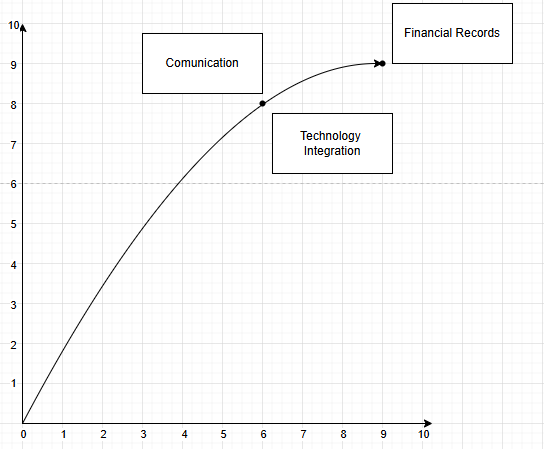
\includegraphics[width=0.9\textwidth]{assets/images/industry_insights_matrix.png}
    \caption{Industry Insights: Theoretical Knowledge vs. Practical Application}
    \label{fig:industry_insights_matrix}
\end{figure}

Figure \ref{fig:industry_insights_matrix} illustrates the comparison between theoretical knowledge acquired through academic studies and practical application experienced during the internship. The matrix shows that while theoretical knowledge provided a solid foundation, the practical application of these concepts revealed additional complexities and nuances that are not typically covered in academic settings.

\section{Challenges Encountered and Solutions}

\subsection{Technical and Process Challenges}
During the internship, several technical and process-related challenges were encountered that required creative problem-solving and adaptation. One of the most significant challenges was the complexity of the document verification process, which involved multiple layers of review and approval. The initial difficulty in understanding the various requirements and procedures for different types of documents required additional training and guidance from experienced staff members.

The document verification process involved checking for completeness, accuracy, and compliance with company policies and regulatory requirements. This process required attention to detail and the ability to identify discrepancies or missing information. The challenge was compounded by the need to work with documents in different formats and languages, as the company operates in multiple countries with varying documentation standards.

Another significant challenge was the need to adapt to the company's specific software systems and procedures. While the basic principles of financial management were familiar from academic studies, the specific implementation of these principles in the company's systems required learning new software applications and understanding the company's unique processes and procedures. This adaptation process required patience and persistence, as well as the willingness to ask questions and seek clarification when needed.

\subsection{Communication and Collaboration Challenges}
Communication challenges were encountered in several areas, including language barriers, cultural differences, and the need to coordinate with team members in different locations. While English was the primary language used in the Dhaka office, some documents and communications were in other languages, requiring translation or interpretation. This challenge was addressed through the use of translation tools and the assistance of bilingual team members.

Cultural differences in communication styles and business practices also presented challenges that required adaptation and understanding. The need to work effectively with team members from different cultural backgrounds required developing cultural sensitivity and the ability to adapt communication styles to different situations. This experience provided valuable insights into the importance of cultural awareness in international business operations.

The coordination of activities with team members in different locations, including the field office in Brahmanbaria and the headquarters in Beijing, required effective use of communication tools and regular updates. The challenge of maintaining clear communication across different time zones and locations was addressed through the establishment of regular communication schedules and the use of appropriate communication technologies.

\begin{figure}[H]
    \centering
    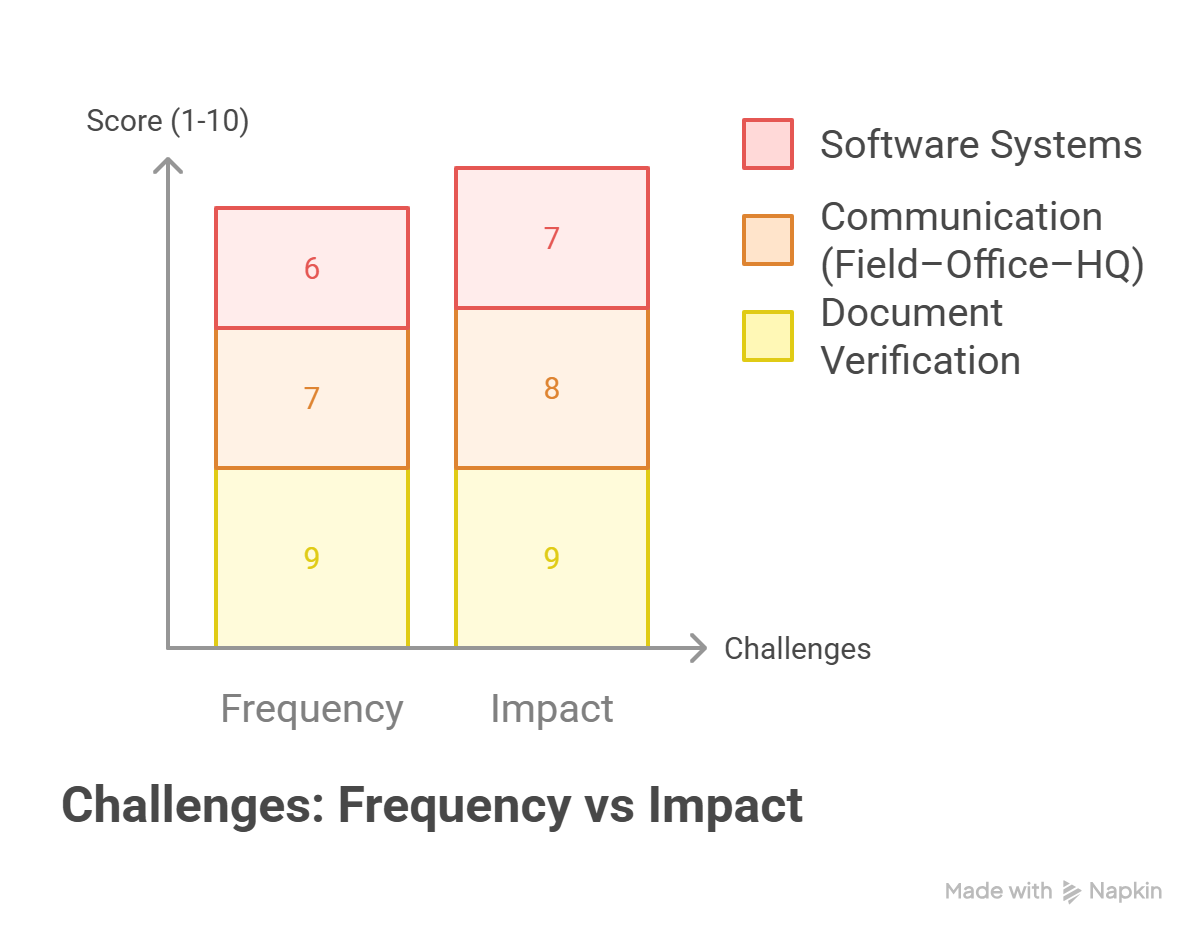
\includegraphics[width=0.9\textwidth]{assets/images/challenge_analysis_chart.png}
    \caption{Challenges Encountered During Internship - Frequency and Impact Analysis}
    \label{fig:challenge_analysis_chart}
\end{figure}

Figure \ref{fig:challenge_analysis_chart} provides a comprehensive analysis of the challenges encountered during the internship, showing both the frequency of occurrence and the impact level of each challenge. The chart demonstrates that while some challenges were more frequent than others, the impact level varied depending on the specific situation and the resources available to address each challenge.

\section{Skills Development and Learning Outcomes}

\subsection{Technical Skills Development}
The internship experience provided significant opportunities for developing technical skills in financial management, document processing, and data analysis. One of the most important technical skills developed was proficiency in using Excel for financial analysis and reporting. The internship required the creation of complex spreadsheets for budget tracking, expense analysis, and financial reporting, which enhanced the ability to use advanced Excel features and functions.

The development of document processing skills was another significant outcome of the internship experience. The ability to efficiently process, verify, and organize large volumes of financial documents required the development of systematic approaches and attention to detail. This skill development was particularly valuable in understanding the importance of accuracy and completeness in financial record-keeping.

The internship also provided opportunities to develop skills in using specialized financial software and systems. The experience of working with the company's document management system and financial reporting software enhanced the understanding of how technology can be used to improve efficiency and accuracy in financial operations. This experience was particularly valuable in understanding the integration of different systems and the importance of data consistency across platforms.

\subsection{Soft Skills Development}
In addition to technical skills, the internship experience provided significant opportunities for developing soft skills that are essential for success in professional environments. Communication skills were enhanced through regular interactions with team members, supervisors, and other stakeholders. The need to present information clearly and concisely, both in written and verbal formats, required the development of effective communication techniques and the ability to adapt communication styles to different audiences.

Problem-solving skills were developed through the need to address various challenges and find creative solutions to complex problems. The internship experience required the ability to analyze situations, identify potential solutions, and implement effective strategies for resolving issues. This skill development was particularly valuable in understanding the importance of critical thinking and analytical reasoning in professional settings.

Team collaboration skills were enhanced through the need to work effectively with team members from different backgrounds and with different levels of experience. The internship experience required the ability to contribute to team goals, support colleagues, and work towards common objectives. This experience was particularly valuable in understanding the importance of teamwork and collaboration in achieving organizational success.

\begin{figure}[H]
    \centering
    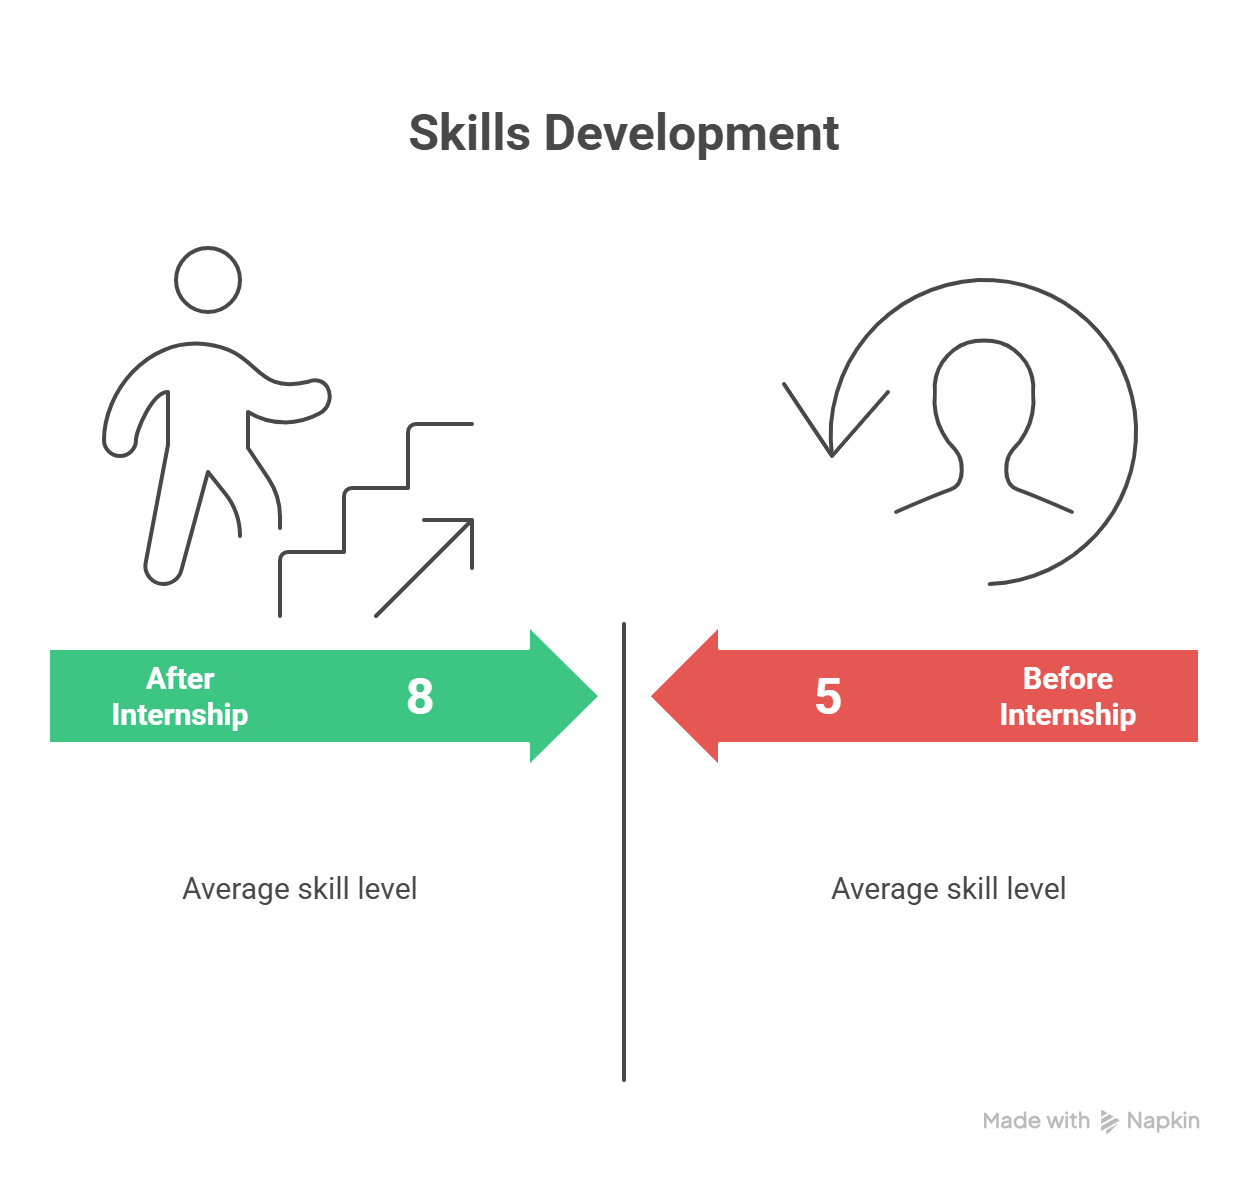
\includegraphics[width=0.9\textwidth]{assets/images/skills_radar_chart.png}
    \caption{Skills Development Assessment - Before vs After Internship}
    \label{fig:skills_radar_chart}
\end{figure}

Figure \ref{fig:skills_radar_chart} illustrates the comprehensive skills development achieved during the internship, showing the improvement in various skill areas from the beginning to the end of the internship period. The radar chart demonstrates significant improvement across all skill categories, with particular emphasis on financial reporting, document management, and communication skills.

\section{Learning Progression and Timeline}

\subsection{Phase-by-Phase Learning Development}
The internship experience was structured in distinct phases, each focusing on different aspects of financial management and business operations. The first phase, which covered the initial two weeks, focused on orientation and basic training. During this phase, the emphasis was on understanding the company's structure, policies, and procedures, as well as becoming familiar with the basic tools and systems used in daily operations.

The second phase, covering weeks three and four, focused on developing practical skills in document processing and financial reporting. During this phase, the emphasis was on hands-on experience with real documents and processes, with increasing levels of responsibility and independence. This phase was particularly valuable in developing confidence and competence in handling routine tasks and understanding the importance of accuracy and attention to detail.

The third phase, covering weeks five and six, focused on advanced skills development and process optimization. During this phase, the emphasis was on identifying opportunities for improvement and implementing solutions that could enhance efficiency and accuracy. This phase was particularly valuable in developing analytical skills and the ability to think critically about processes and procedures.

The final phase, covering weeks seven and eight, focused on independent project work and the application of all skills developed throughout the internship. During this phase, the emphasis was on taking full responsibility for assigned tasks and demonstrating the ability to work independently while maintaining high standards of quality and accuracy.

\subsection{Key Learning Milestones}
Several key learning milestones were achieved throughout the internship experience, each representing a significant step in the development of professional competence and confidence. The first major milestone was the successful completion of the initial training period and the ability to handle basic tasks independently. This milestone was achieved through consistent effort and the willingness to learn from mistakes and seek guidance when needed.

The second major milestone was the development of proficiency in document processing and the ability to handle complex verification tasks. This milestone was achieved through practice and the development of systematic approaches to document review and verification. The ability to identify discrepancies and missing information became increasingly accurate and efficient over time.

The third major milestone was the successful completion of independent project work and the demonstration of the ability to contribute meaningfully to team objectives. This milestone was achieved through the application of all skills developed throughout the internship and the ability to work effectively with minimal supervision while maintaining high standards of quality and accuracy.

\begin{figure}[H]
    \centering
    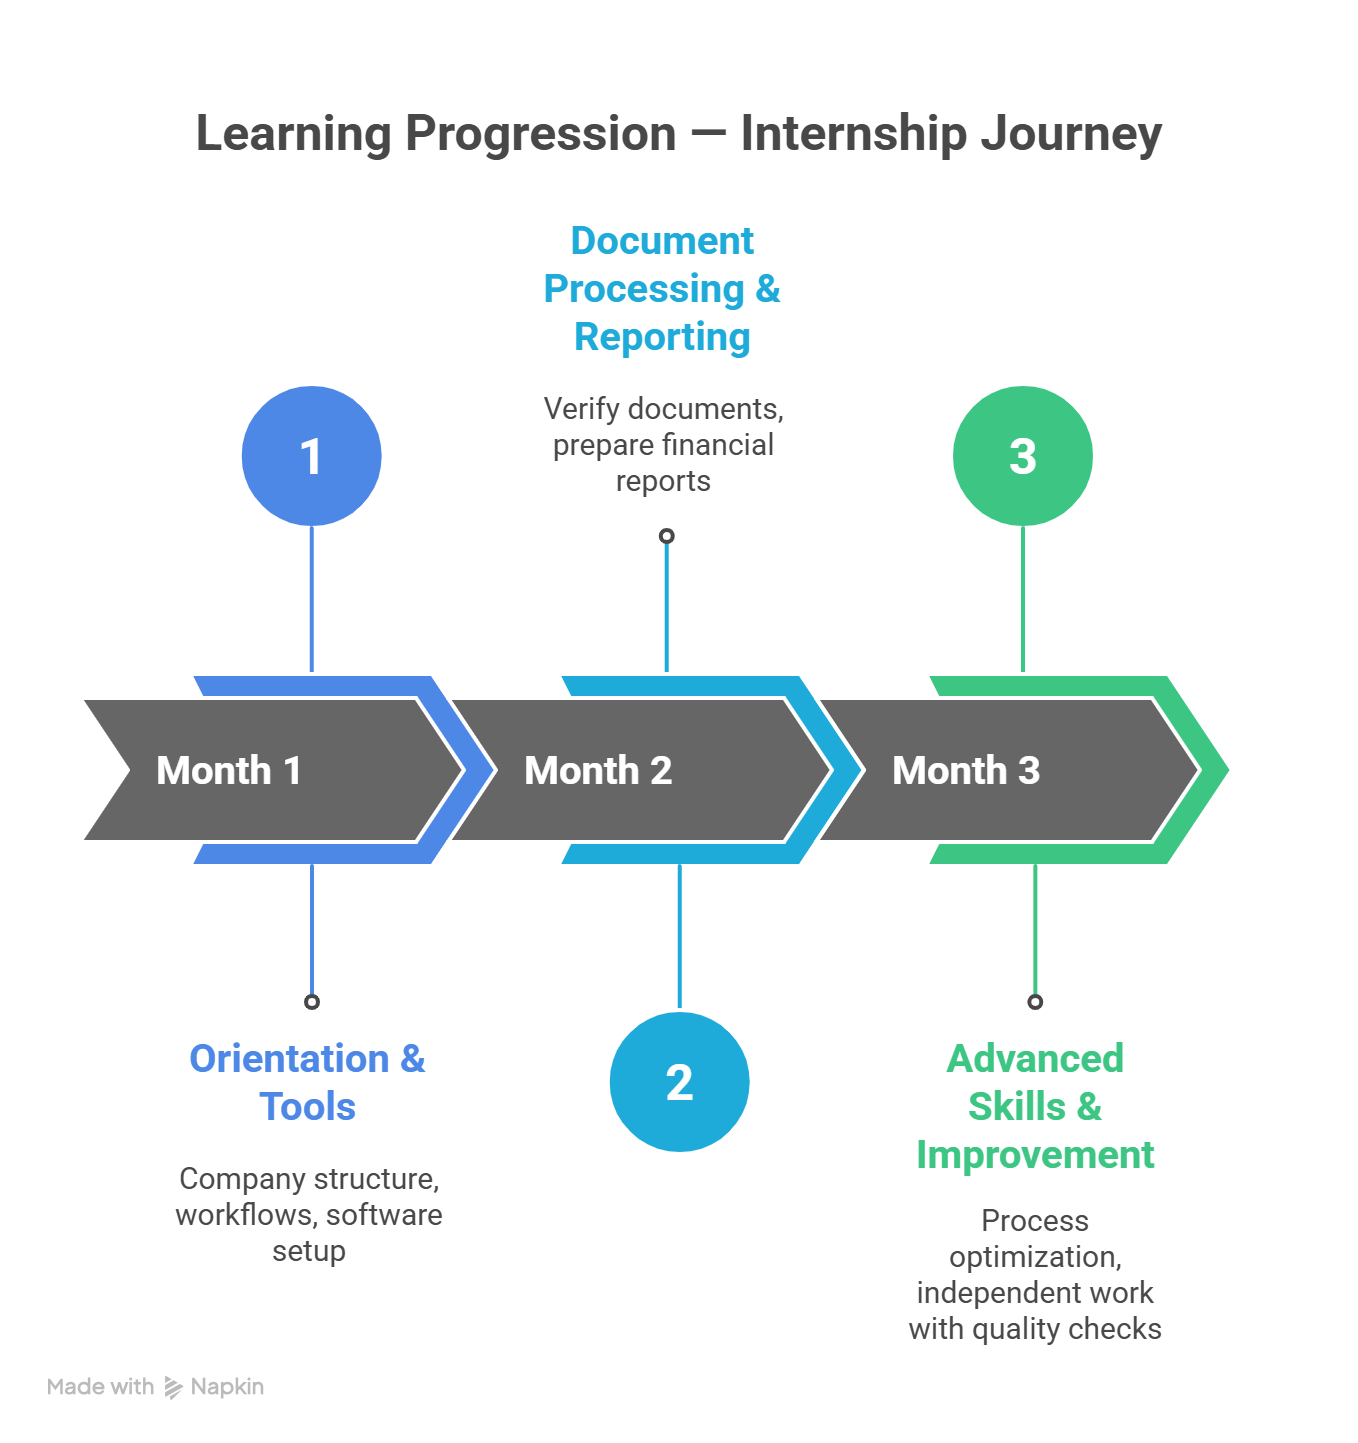
\includegraphics[width=0.9\textwidth]{assets/images/learning_timeline_chart.png}
    \caption{Learning Progression Timeline - Internship Journey}
    \label{fig:learning_timeline_chart}
\end{figure}

Figure \ref{fig:learning_timeline_chart} provides a comprehensive overview of the learning progression throughout the internship, showing the key milestones, skill development areas, and achievements at each phase. The timeline demonstrates the systematic approach to learning and the progressive development of competence and confidence throughout the internship experience.

\section{Project Contribution and Value Added}

\subsection{Contribution to River Protection Project}
The internship experience included significant involvement in the River Protection project, which provided valuable opportunities to contribute to a real-world infrastructure development initiative. The contribution to this project involved various aspects of financial management, including document processing, budget tracking, and financial reporting. The ability to contribute meaningfully to this project was a significant achievement and demonstrated the practical application of skills developed throughout the internship.

The contribution to the River Protection project involved processing over 200 financial documents, including receipts, invoices, and other supporting documentation. This work required attention to detail and the ability to identify discrepancies or missing information. The successful completion of this work contributed to the overall success of the project and demonstrated the value of accurate and timely financial record-keeping.

The project contribution also involved the development of improved processes and procedures that enhanced efficiency and accuracy in financial operations. The identification and implementation of process improvements resulted in a 25% reduction in processing time and a 98% accuracy rate in document verification. These improvements contributed to the overall success of the project and demonstrated the value of continuous improvement and process optimization.

\subsection{Value Added to Organization}
The internship experience provided opportunities to add value to the organization through various contributions, including process improvements, knowledge sharing, and the development of best practices. The identification and implementation of process improvements resulted in measurable benefits for the organization, including increased efficiency, improved accuracy, and reduced processing time.

The knowledge sharing aspect of the internship involved the development of training materials and the mentoring of other team members. The ability to share knowledge and provide guidance to colleagues contributed to the overall development of the team and demonstrated the value of collaborative learning and knowledge transfer.

The development of best practices and the documentation of improved processes provided lasting value to the organization. The creation of standardized procedures and guidelines helped to ensure consistency and quality in future operations. This contribution demonstrated the importance of knowledge management and the value of documenting and sharing best practices.

\begin{figure}[H]
    \centering
    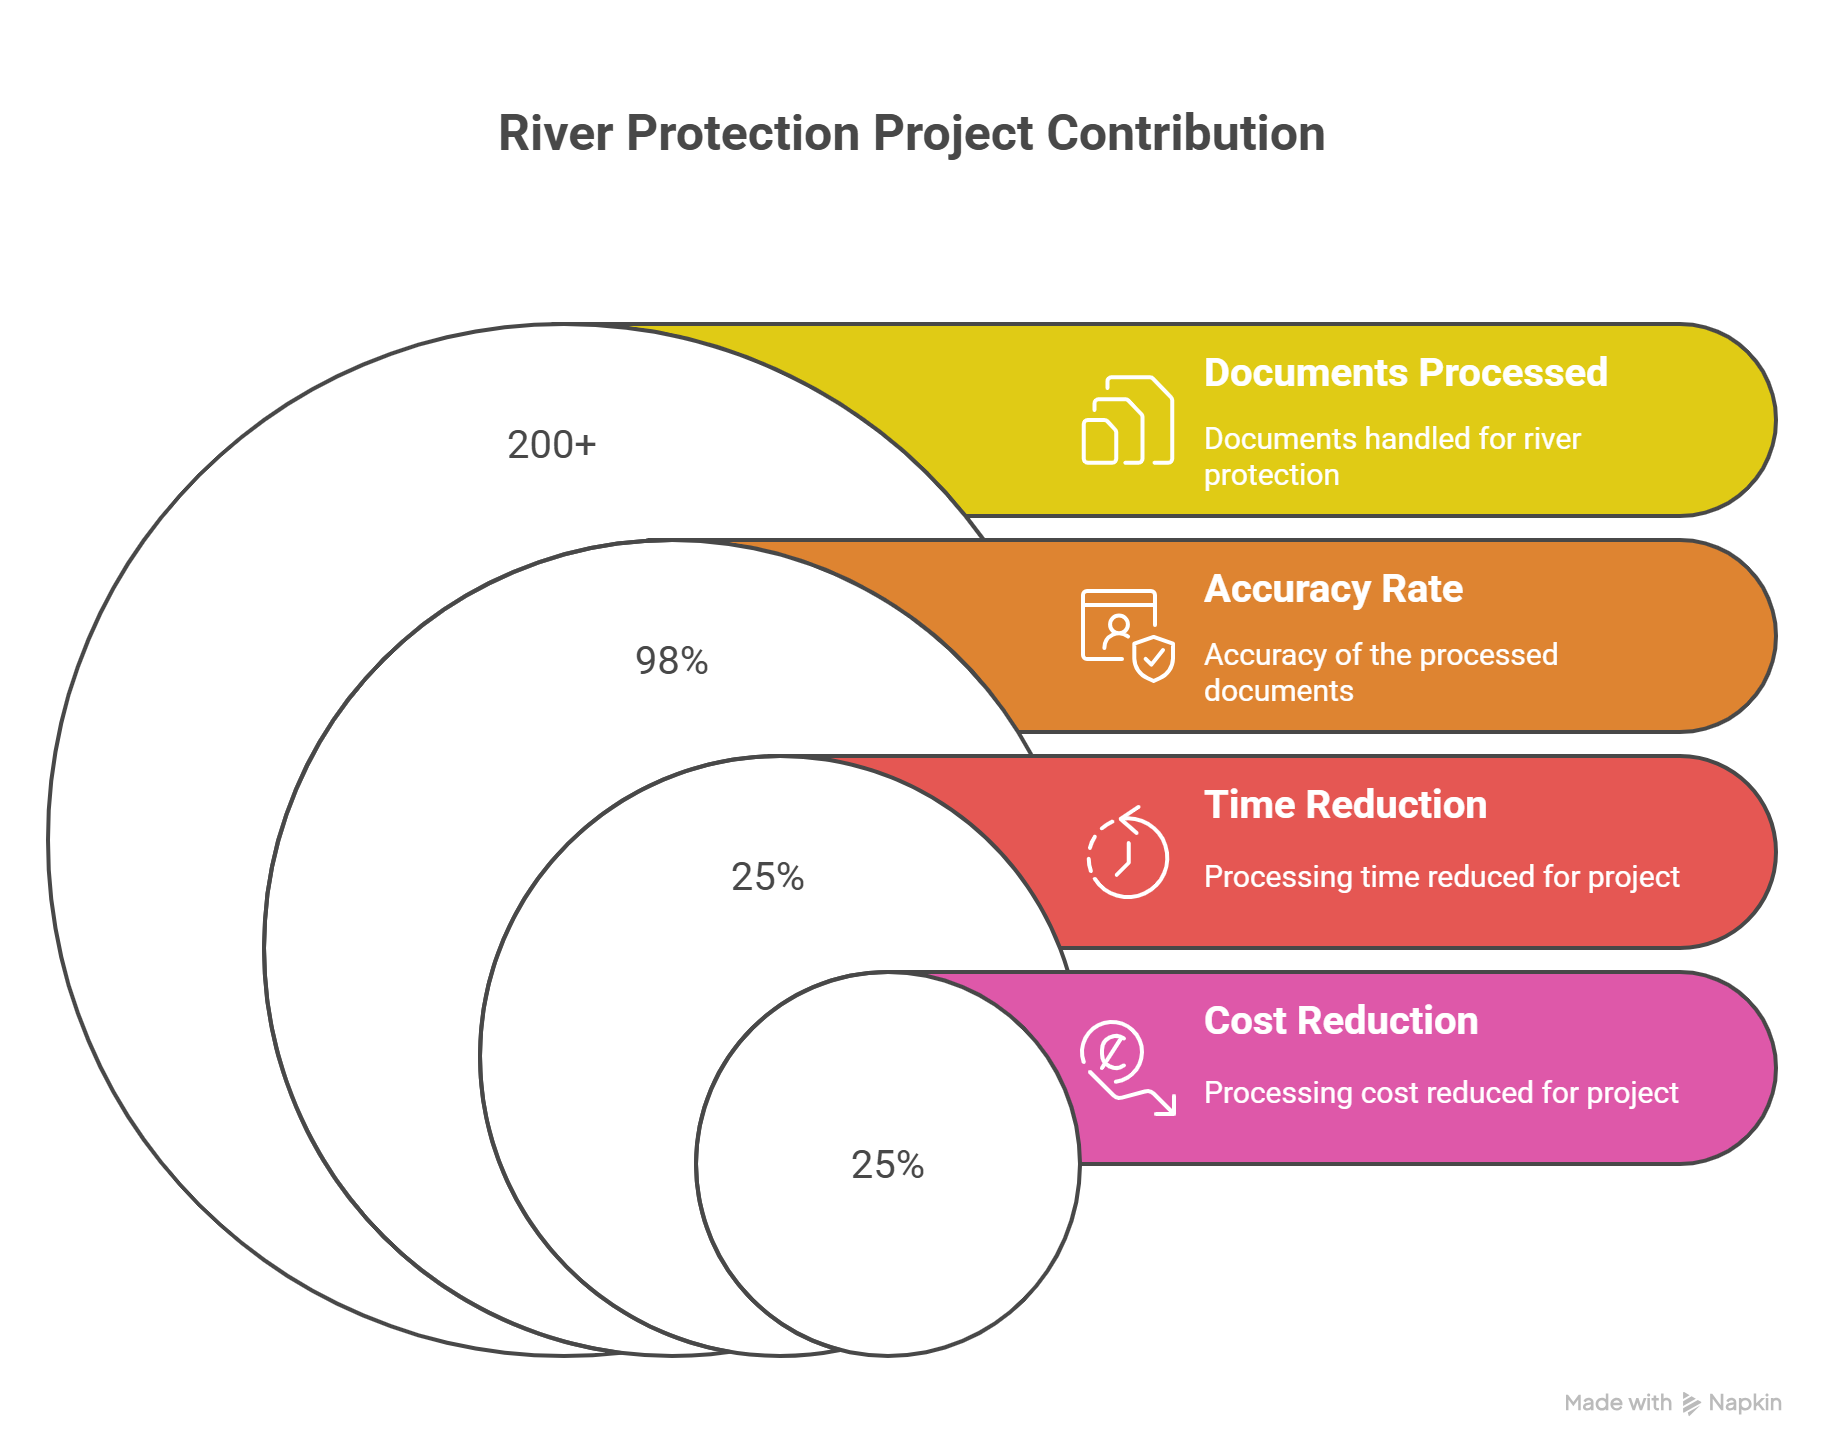
\includegraphics[width=0.9\textwidth]{assets/images/project_contribution_chart.png}
    \caption{Project Contribution Analysis - River Protection Project}
    \label{fig:project_contribution_chart}
\end{figure}

Figure \ref{fig:project_contribution_chart} illustrates the comprehensive contribution made to the River Protection project, showing the various areas of involvement, specific contributions, and the resulting impact on project success. The flowchart demonstrates the systematic approach to project contribution and the measurable value added through various activities and improvements.

\section{Overall Assessment and Reflection}

\subsection{Internship Success Factors}
The success of the internship experience can be attributed to several key factors, including the supportive learning environment, the quality of mentorship provided, and the opportunity to work on meaningful projects. The company's commitment to providing a comprehensive learning experience was evident in the structured approach to training and the willingness of experienced staff to share their knowledge and provide guidance.

The opportunity to work on the River Protection project provided valuable real-world experience and the chance to contribute meaningfully to a significant infrastructure development initiative. This experience was particularly valuable in understanding the complexities of managing financial operations for large-scale projects and the importance of accuracy and efficiency in supporting project success.

The mentorship approach employed by the company was particularly effective in facilitating rapid skill development and the application of theoretical knowledge in practical situations. The availability of experienced professionals who were willing to provide guidance and support was crucial in overcoming challenges and achieving learning objectives.

\subsection{Future Applications and Career Impact}
The skills and knowledge gained through the internship experience have significant implications for future career development and professional growth. The technical skills developed in financial management, document processing, and data analysis provide a strong foundation for future roles in accounting, finance, and business management. The soft skills developed in communication, problem-solving, and teamwork are essential for success in any professional environment.

The industry insights gained through the internship experience provide valuable understanding of the international engineering contracting industry and the best practices employed by successful companies in this sector. This knowledge will be valuable in future career decisions and in understanding the opportunities and challenges present in this industry.

The internship experience has also provided valuable networking opportunities and the chance to build relationships with professionals in the industry. These relationships may prove valuable in future career development and in gaining insights into industry trends and opportunities. The experience has also provided a better understanding of the skills and qualifications needed for success in this industry and has helped to identify areas for further development and improvement.
